% Options for packages loaded elsewhere
\PassOptionsToPackage{unicode}{hyperref}
\PassOptionsToPackage{hyphens}{url}
%
\documentclass[
]{article}
\usepackage{amsmath,amssymb}
\usepackage{iftex}
\ifPDFTeX
  \usepackage[T1]{fontenc}
  \usepackage[utf8]{inputenc}
  \usepackage{textcomp} % provide euro and other symbols
\else % if luatex or xetex
  \usepackage{unicode-math} % this also loads fontspec
  \defaultfontfeatures{Scale=MatchLowercase}
  \defaultfontfeatures[\rmfamily]{Ligatures=TeX,Scale=1}
\fi
\usepackage{lmodern}
\ifPDFTeX\else
  % xetex/luatex font selection
\fi
% Use upquote if available, for straight quotes in verbatim environments
\IfFileExists{upquote.sty}{\usepackage{upquote}}{}
\IfFileExists{microtype.sty}{% use microtype if available
  \usepackage[]{microtype}
  \UseMicrotypeSet[protrusion]{basicmath} % disable protrusion for tt fonts
}{}
\makeatletter
\@ifundefined{KOMAClassName}{% if non-KOMA class
  \IfFileExists{parskip.sty}{%
    \usepackage{parskip}
  }{% else
    \setlength{\parindent}{0pt}
    \setlength{\parskip}{6pt plus 2pt minus 1pt}}
}{% if KOMA class
  \KOMAoptions{parskip=half}}
\makeatother
\usepackage{xcolor}
\usepackage[margin=1in]{geometry}
\usepackage{color}
\usepackage{fancyvrb}
\newcommand{\VerbBar}{|}
\newcommand{\VERB}{\Verb[commandchars=\\\{\}]}
\DefineVerbatimEnvironment{Highlighting}{Verbatim}{commandchars=\\\{\}}
% Add ',fontsize=\small' for more characters per line
\usepackage{framed}
\definecolor{shadecolor}{RGB}{248,248,248}
\newenvironment{Shaded}{\begin{snugshade}}{\end{snugshade}}
\newcommand{\AlertTok}[1]{\textcolor[rgb]{0.94,0.16,0.16}{#1}}
\newcommand{\AnnotationTok}[1]{\textcolor[rgb]{0.56,0.35,0.01}{\textbf{\textit{#1}}}}
\newcommand{\AttributeTok}[1]{\textcolor[rgb]{0.13,0.29,0.53}{#1}}
\newcommand{\BaseNTok}[1]{\textcolor[rgb]{0.00,0.00,0.81}{#1}}
\newcommand{\BuiltInTok}[1]{#1}
\newcommand{\CharTok}[1]{\textcolor[rgb]{0.31,0.60,0.02}{#1}}
\newcommand{\CommentTok}[1]{\textcolor[rgb]{0.56,0.35,0.01}{\textit{#1}}}
\newcommand{\CommentVarTok}[1]{\textcolor[rgb]{0.56,0.35,0.01}{\textbf{\textit{#1}}}}
\newcommand{\ConstantTok}[1]{\textcolor[rgb]{0.56,0.35,0.01}{#1}}
\newcommand{\ControlFlowTok}[1]{\textcolor[rgb]{0.13,0.29,0.53}{\textbf{#1}}}
\newcommand{\DataTypeTok}[1]{\textcolor[rgb]{0.13,0.29,0.53}{#1}}
\newcommand{\DecValTok}[1]{\textcolor[rgb]{0.00,0.00,0.81}{#1}}
\newcommand{\DocumentationTok}[1]{\textcolor[rgb]{0.56,0.35,0.01}{\textbf{\textit{#1}}}}
\newcommand{\ErrorTok}[1]{\textcolor[rgb]{0.64,0.00,0.00}{\textbf{#1}}}
\newcommand{\ExtensionTok}[1]{#1}
\newcommand{\FloatTok}[1]{\textcolor[rgb]{0.00,0.00,0.81}{#1}}
\newcommand{\FunctionTok}[1]{\textcolor[rgb]{0.13,0.29,0.53}{\textbf{#1}}}
\newcommand{\ImportTok}[1]{#1}
\newcommand{\InformationTok}[1]{\textcolor[rgb]{0.56,0.35,0.01}{\textbf{\textit{#1}}}}
\newcommand{\KeywordTok}[1]{\textcolor[rgb]{0.13,0.29,0.53}{\textbf{#1}}}
\newcommand{\NormalTok}[1]{#1}
\newcommand{\OperatorTok}[1]{\textcolor[rgb]{0.81,0.36,0.00}{\textbf{#1}}}
\newcommand{\OtherTok}[1]{\textcolor[rgb]{0.56,0.35,0.01}{#1}}
\newcommand{\PreprocessorTok}[1]{\textcolor[rgb]{0.56,0.35,0.01}{\textit{#1}}}
\newcommand{\RegionMarkerTok}[1]{#1}
\newcommand{\SpecialCharTok}[1]{\textcolor[rgb]{0.81,0.36,0.00}{\textbf{#1}}}
\newcommand{\SpecialStringTok}[1]{\textcolor[rgb]{0.31,0.60,0.02}{#1}}
\newcommand{\StringTok}[1]{\textcolor[rgb]{0.31,0.60,0.02}{#1}}
\newcommand{\VariableTok}[1]{\textcolor[rgb]{0.00,0.00,0.00}{#1}}
\newcommand{\VerbatimStringTok}[1]{\textcolor[rgb]{0.31,0.60,0.02}{#1}}
\newcommand{\WarningTok}[1]{\textcolor[rgb]{0.56,0.35,0.01}{\textbf{\textit{#1}}}}
\usepackage{graphicx}
\makeatletter
\newsavebox\pandoc@box
\newcommand*\pandocbounded[1]{% scales image to fit in text height/width
  \sbox\pandoc@box{#1}%
  \Gscale@div\@tempa{\textheight}{\dimexpr\ht\pandoc@box+\dp\pandoc@box\relax}%
  \Gscale@div\@tempb{\linewidth}{\wd\pandoc@box}%
  \ifdim\@tempb\p@<\@tempa\p@\let\@tempa\@tempb\fi% select the smaller of both
  \ifdim\@tempa\p@<\p@\scalebox{\@tempa}{\usebox\pandoc@box}%
  \else\usebox{\pandoc@box}%
  \fi%
}
% Set default figure placement to htbp
\def\fps@figure{htbp}
\makeatother
\setlength{\emergencystretch}{3em} % prevent overfull lines
\providecommand{\tightlist}{%
  \setlength{\itemsep}{0pt}\setlength{\parskip}{0pt}}
\setcounter{secnumdepth}{5}
\usepackage{bookmark}
\IfFileExists{xurl.sty}{\usepackage{xurl}}{} % add URL line breaks if available
\urlstyle{same}
\hypersetup{
  pdftitle={Homework 1},
  pdfauthor={Santiago Ruiz, Nikita Karetnikov,},
  hidelinks,
  pdfcreator={LaTeX via pandoc}}

\title{\textbf{Homework 1}}
\author{Santiago Ruiz, Nikita Karetnikov,}
\date{2025-03-19}

\begin{document}
\maketitle

\section{Exercise 1}\label{exercise-1}

In this exercise, we are asked to calculate the limits for a system of
number representations with the following parameters:

\begin{itemize}
\tightlist
\item
  \(b = 10\) base
\item
  \(m = 3\) mantissa length
\item
  \(e_{\min} = -3\)
\item
  \(e_{\max} = 4\)
\end{itemize}

To calculate the required numbers we would need the following formula:

\[
x = (-1)^{w_0} b^e \sum_{i=1}^{m} u_i b^{-i}
\] Let us implement it in R:

\begin{Shaded}
\begin{Highlighting}[]
\NormalTok{calculate }\OtherTok{\textless{}{-}} \ControlFlowTok{function}\NormalTok{(w0, b, e, u,m)\{}
\NormalTok{  mantissa }\OtherTok{\textless{}{-}} \DecValTok{0}   
  
  \ControlFlowTok{for}\NormalTok{ (i }\ControlFlowTok{in} \DecValTok{1}\SpecialCharTok{:}\NormalTok{m) \{}
\NormalTok{    mantissa }\OtherTok{\textless{}{-}}\NormalTok{ mantissa }\SpecialCharTok{+}\NormalTok{ u[i] }\SpecialCharTok{*}\NormalTok{ b}\SpecialCharTok{\^{}}\NormalTok{(}\SpecialCharTok{{-}}\NormalTok{i)}
\NormalTok{  \}}
  
\NormalTok{  x }\OtherTok{\textless{}{-}}\NormalTok{ (}\SpecialCharTok{{-}}\DecValTok{1}\NormalTok{)}\SpecialCharTok{\^{}}\NormalTok{w0 }\SpecialCharTok{*}\NormalTok{ b}\SpecialCharTok{\^{}}\NormalTok{e }\SpecialCharTok{*}\NormalTok{ mantissa}
  
  \FunctionTok{return}\NormalTok{(x)}
\NormalTok{\}}
\end{Highlighting}
\end{Shaded}

Good! Now we will be able to determine the required numbers.

\subsection{Determine the largest floating point
number}\label{determine-the-largest-floating-point-number}

We start with the largest floating point number. We assume that the
largest number should have:

\begin{itemize}
\tightlist
\item
  the largest possible exponent
\item
  mantissa with the largest digits in this system (which should be equal
  to b-1)
\end{itemize}

\begin{Shaded}
\begin{Highlighting}[]
\NormalTok{b }\OtherTok{\textless{}{-}} \DecValTok{10}  
\NormalTok{m }\OtherTok{\textless{}{-}} \DecValTok{3}

\NormalTok{e\_min }\OtherTok{\textless{}{-}} \SpecialCharTok{{-}}\DecValTok{3}  
\NormalTok{e\_max }\OtherTok{\textless{}{-}} \DecValTok{4}


\NormalTok{x\_max }\OtherTok{\textless{}{-}} \FunctionTok{calculate}\NormalTok{(}\AttributeTok{w0=}\DecValTok{0}\NormalTok{, }\AttributeTok{b=}\NormalTok{b, }\AttributeTok{e=}\NormalTok{e\_max, }\AttributeTok{u=} \FunctionTok{rep}\NormalTok{(b}\DecValTok{{-}1}\NormalTok{, m),}\AttributeTok{m=}\NormalTok{m)}
\FunctionTok{print}\NormalTok{(x\_max)}
\end{Highlighting}
\end{Shaded}

\begin{verbatim}
## [1] 9990
\end{verbatim}

\subsection{Determine the smallest positive floating point
number}\label{determine-the-smallest-positive-floating-point-number}

Now we should determine the smallest positive floating point number. We
assume that the largest number should have:

\begin{itemize}
\tightlist
\item
  the smallest possible exponent
\item
  mantissa with the smallest digits in this system (which should be
  equal to 0)
\end{itemize}

But since mantissa should start with non-zero we set its digits to
{[}1,0,0{]} :

\begin{Shaded}
\begin{Highlighting}[]
\NormalTok{x\_min }\OtherTok{\textless{}{-}} \FunctionTok{calculate}\NormalTok{(}\AttributeTok{w0 =} \DecValTok{0}\NormalTok{, }\AttributeTok{b =}\NormalTok{ b, }\AttributeTok{e =}\NormalTok{ e\_min, }\AttributeTok{u =} \FunctionTok{c}\NormalTok{(}\DecValTok{1}\NormalTok{,}\DecValTok{0}\NormalTok{,}\DecValTok{0}\NormalTok{), }\AttributeTok{m =}\NormalTok{ m)}

\FunctionTok{print}\NormalTok{(x\_min)}
\end{Highlighting}
\end{Shaded}

\begin{verbatim}
## [1] 1e-04
\end{verbatim}

\subsection{Determine the largest floating point number smaller than
one.}\label{determine-the-largest-floating-point-number-smaller-than-one.}

Now we should find the number that approaches value of 1, but that is
smaller then one.

We set: - exponent to 0 - mantissa to have largest digits in this system
(which should be equal to b-1)

\begin{Shaded}
\begin{Highlighting}[]
\NormalTok{x\_max\_2 }\OtherTok{\textless{}{-}} \FunctionTok{calculate}\NormalTok{(}\AttributeTok{w0 =} \DecValTok{0}\NormalTok{, }\AttributeTok{b =}\NormalTok{ b, }\AttributeTok{e =} \DecValTok{0}\NormalTok{, }\AttributeTok{u=} \FunctionTok{rep}\NormalTok{(b}\DecValTok{{-}1}\NormalTok{, m), }\AttributeTok{m =}\NormalTok{ m)}
\FunctionTok{print}\NormalTok{(x\_max\_2)}
\end{Highlighting}
\end{Shaded}

\begin{verbatim}
## [1] 0.999
\end{verbatim}

\subsection{Determine the smallest floating point number greater than
one}\label{determine-the-smallest-floating-point-number-greater-than-one}

Now similarly we should find the number that is closest to one, but is
bigger than one.

We set: - exponent to 0 - mantissa digits to be equal to {[}1,0,1{]}

\begin{Shaded}
\begin{Highlighting}[]
\NormalTok{x\_min\_2 }\OtherTok{\textless{}{-}} \FunctionTok{calculate}\NormalTok{(}\AttributeTok{w0 =} \DecValTok{0}\NormalTok{, }\AttributeTok{b =}\NormalTok{ b, }\AttributeTok{e =} \DecValTok{1}\NormalTok{, }\AttributeTok{u =} \FunctionTok{c}\NormalTok{(}\DecValTok{1}\NormalTok{,}\DecValTok{0}\NormalTok{,}\DecValTok{1}\NormalTok{), }\AttributeTok{m =}\NormalTok{ m)}
\FunctionTok{print}\NormalTok{(x\_min\_2)}
\end{Highlighting}
\end{Shaded}

\begin{verbatim}
## [1] 1.01
\end{verbatim}

\section{Exercise 2}\label{exercise-2}

In this exercise we need to understand the limits or R number
representation system by running experiments with convergence of the
series.

\subsection{For which n does the loop stop? (practical
part)}\label{for-which-n-does-the-loop-stop-practical-part}

We first implement convergence in R. We run the loop until the
difference between \(S_{n+1}\) and \(S_n\) becomes smaller than the
smallest number that R can distinguish. .

\begin{Shaded}
\begin{Highlighting}[]
\NormalTok{S\_n\_prev }\OtherTok{\textless{}{-}} \SpecialCharTok{{-}}\DecValTok{1}  
\NormalTok{S\_n }\OtherTok{\textless{}{-}} \DecValTok{0}
\NormalTok{n }\OtherTok{\textless{}{-}} \DecValTok{0}  

\ControlFlowTok{while}\NormalTok{ (}\FunctionTok{abs}\NormalTok{(S\_n }\SpecialCharTok{{-}}\NormalTok{ S\_n\_prev) }\SpecialCharTok{\textgreater{}}\NormalTok{ .Machine}\SpecialCharTok{$}\NormalTok{double.eps)\{ }
\NormalTok{  n }\OtherTok{\textless{}{-}}\NormalTok{  n }\SpecialCharTok{+} \DecValTok{1}
\NormalTok{  S\_n\_prev  }\OtherTok{\textless{}{-}}\NormalTok{ S\_n}
\NormalTok{  S\_n }\OtherTok{\textless{}{-}}\NormalTok{ S\_n\_prev }\SpecialCharTok{+} \DecValTok{2}\SpecialCharTok{\^{}}\NormalTok{(}\SpecialCharTok{{-}}\DecValTok{2} \SpecialCharTok{*}\NormalTok{ n)}
\NormalTok{\}}

\FunctionTok{cat}\NormalTok{(}\StringTok{"Loop stops at n ="}\NormalTok{,n)}
\end{Highlighting}
\end{Shaded}

\begin{verbatim}
## Loop stops at n = 26
\end{verbatim}

\subsection{For which n does the loop stop? (theoretical
part)}\label{for-which-n-does-the-loop-stop-theoretical-part}

Now we need to theoretically approximate the value of \(n\) at which the
loop stops. We observe that the convergence of our series resembles the
formula used to represent numbers in R.

\[
\sum_{i=1}^{\infty} 2^{-2i} 
\quad\quad\quad\quad
x = (-1)^{w_0} b^{e} \sum_{i=1}^{m} u_i b^{-i}
\] Let us remind ourselves what is mantissa length and base in R is:

\begin{Shaded}
\begin{Highlighting}[]
\NormalTok{m }\OtherTok{\textless{}{-}}\NormalTok{  .Machine}\SpecialCharTok{$}\NormalTok{double.digits}
\FunctionTok{cat}\NormalTok{(}\StringTok{"Mantissa length (m):"}\NormalTok{, m, }\StringTok{"}\SpecialCharTok{\textbackslash{}n}\StringTok{"}\NormalTok{)}
\end{Highlighting}
\end{Shaded}

\begin{verbatim}
## Mantissa length (m): 53
\end{verbatim}

\begin{Shaded}
\begin{Highlighting}[]
\NormalTok{b }\OtherTok{\textless{}{-}}\NormalTok{  .Machine}\SpecialCharTok{$}\NormalTok{double.base}
\FunctionTok{cat}\NormalTok{(}\StringTok{"Base (b):"}\NormalTok{, b, }\StringTok{"}\SpecialCharTok{\textbackslash{}n}\StringTok{"}\NormalTok{)}
\end{Highlighting}
\end{Shaded}

\begin{verbatim}
## Base (b): 2
\end{verbatim}

With each iteration, the summation approaches its limit more closely,
but the increment decreases rapidly (each term is \(2^{-2i}\)). Due to
floating-point representation limits in R (with a mantissa length
\(m = 53\) bits for double precision), the smallest distinguishable
difference around 1 is about \(2^{-53}\).

The summation stops updating numerically when the next term \(2^{-2n}\)
becomes smaller than this limit:

\[
2^{-2n} \approx 2^{-m} \quad \Rightarrow \quad n = \frac{m}{2} = \frac{53}{2} = 26.5
\] 26.5 is quite close to the practical stopping point we found earlier.

\section{Exercise 3}\label{exercise-3}

In this exercise we are asked to approximate exp(x) using Taylor series.

\[
\exp(x) = \sum_{i=0}^{\infty} \frac{x^i}{i!}
\]

\subsection{(i)}\label{i}

We implement an algorithm in R that approximates the exponential
function \(\exp(x)\) using the Taylor series expansion. The algorithm
iteratively adds terms from the Taylor series until the absolute value
of the next summand is smaller than
\texttt{.Machine\$double.eps\textasciicircum(1/2)} times the absolute
value of the current approximation.

We run it to identify how many summands we need to approximate
\(\exp(x=10)\)

\begin{Shaded}
\begin{Highlighting}[]
\NormalTok{calculate\_exp }\OtherTok{\textless{}{-}} \ControlFlowTok{function}\NormalTok{(X)\{}
\NormalTok{  term }\OtherTok{\textless{}{-}} \DecValTok{1}              
\NormalTok{  sum }\OtherTok{\textless{}{-}}\NormalTok{ term            }
\NormalTok{  n }\OtherTok{\textless{}{-}} \DecValTok{0}                 
\NormalTok{  epsilon }\OtherTok{\textless{}{-}}\NormalTok{ .Machine}\SpecialCharTok{$}\NormalTok{double.eps}\SpecialCharTok{\^{}}\NormalTok{(}\DecValTok{1}\SpecialCharTok{/}\DecValTok{2}\NormalTok{)  }
    
    
  \ControlFlowTok{while}\NormalTok{ (}\FunctionTok{abs}\NormalTok{(term) }\SpecialCharTok{\textgreater{}}\NormalTok{ epsilon }\SpecialCharTok{*} \FunctionTok{abs}\NormalTok{(sum)) \{}
    
\NormalTok{    n }\OtherTok{\textless{}{-}}\NormalTok{ n }\SpecialCharTok{+} \DecValTok{1}
\NormalTok{    term }\OtherTok{\textless{}{-}}\NormalTok{ (X}\SpecialCharTok{\^{}}\NormalTok{n) }\SpecialCharTok{/} \FunctionTok{factorial}\NormalTok{(n)  }
\NormalTok{    sum }\OtherTok{\textless{}{-}}\NormalTok{ sum }\SpecialCharTok{+}\NormalTok{ term}
  

\NormalTok{  \} }
  \FunctionTok{return}\NormalTok{(sum)}
  
\NormalTok{\}}

\NormalTok{X }\OtherTok{\textless{}{-}} \DecValTok{40}



\FunctionTok{cat}\NormalTok{(}\StringTok{"Our function:"}\NormalTok{, }\FunctionTok{calculate\_exp}\NormalTok{(X), }\StringTok{"}\SpecialCharTok{\textbackslash{}n}\StringTok{"}\NormalTok{)}
\end{Highlighting}
\end{Shaded}

\begin{verbatim}
## Our function: 2.353853e+17
\end{verbatim}

\begin{Shaded}
\begin{Highlighting}[]
\FunctionTok{cat}\NormalTok{(}\StringTok{"R actual function"}\NormalTok{, }\FunctionTok{exp}\NormalTok{(X), }\StringTok{"}\SpecialCharTok{\textbackslash{}n}\StringTok{"}\NormalTok{)}
\end{Highlighting}
\end{Shaded}

\begin{verbatim}
## R actual function 2.353853e+17
\end{verbatim}

Looks that our implemented function closely matches R's built-in
calculation of the exponential function. the exponent.

\subsection{(ii)}\label{ii}

Next, we evaluate the approximation for various values of \(X\), both
positive and negative. We calculate the MAPE for values ranging from
\(-20\) to \(200\).

\begin{Shaded}
\begin{Highlighting}[]
\NormalTok{X\_values }\OtherTok{\textless{}{-}} \FunctionTok{seq}\NormalTok{(}\SpecialCharTok{{-}}\DecValTok{20}\NormalTok{, }\DecValTok{200}\NormalTok{, }\AttributeTok{by=}\DecValTok{1}\NormalTok{)}
\NormalTok{errors }\OtherTok{\textless{}{-}} \FunctionTok{numeric}\NormalTok{(}\FunctionTok{length}\NormalTok{(X\_values)) }

\ControlFlowTok{for}\NormalTok{ (i }\ControlFlowTok{in} \FunctionTok{seq\_along}\NormalTok{(X\_values)) \{}
\NormalTok{  X }\OtherTok{\textless{}{-}}\NormalTok{ X\_values[i]}
  
  
\NormalTok{  mape }\OtherTok{\textless{}{-}} \FunctionTok{mean}\NormalTok{(}\FunctionTok{abs}\NormalTok{((}\FunctionTok{exp}\NormalTok{(X) }\SpecialCharTok{{-}} \FunctionTok{calculate\_exp}\NormalTok{(X)) }\SpecialCharTok{/} \FunctionTok{exp}\NormalTok{(X))) }\SpecialCharTok{*} \DecValTok{100}

  
  
\NormalTok{  errors[i] }\OtherTok{\textless{}{-}}\NormalTok{ mape  }
\NormalTok{\}}


\FunctionTok{plot}\NormalTok{(X\_values, errors, }\AttributeTok{type =} \StringTok{"b"}\NormalTok{, }\AttributeTok{col =} \StringTok{"blue"}\NormalTok{,}
     \AttributeTok{xlab =} \StringTok{"X Value"}\NormalTok{, }\AttributeTok{ylab =} \StringTok{"Error"}\NormalTok{,}
     \AttributeTok{main =} \StringTok{"Error of Taylor Approximation of exp(X)"}\NormalTok{,}
     \AttributeTok{ylim =} \FunctionTok{c}\NormalTok{(}\DecValTok{0}\NormalTok{, }\DecValTok{10}\NormalTok{))  }\CommentTok{\# Adjust these limits as needed for your data}
\FunctionTok{grid}\NormalTok{()}
\end{Highlighting}
\end{Shaded}

\pandocbounded{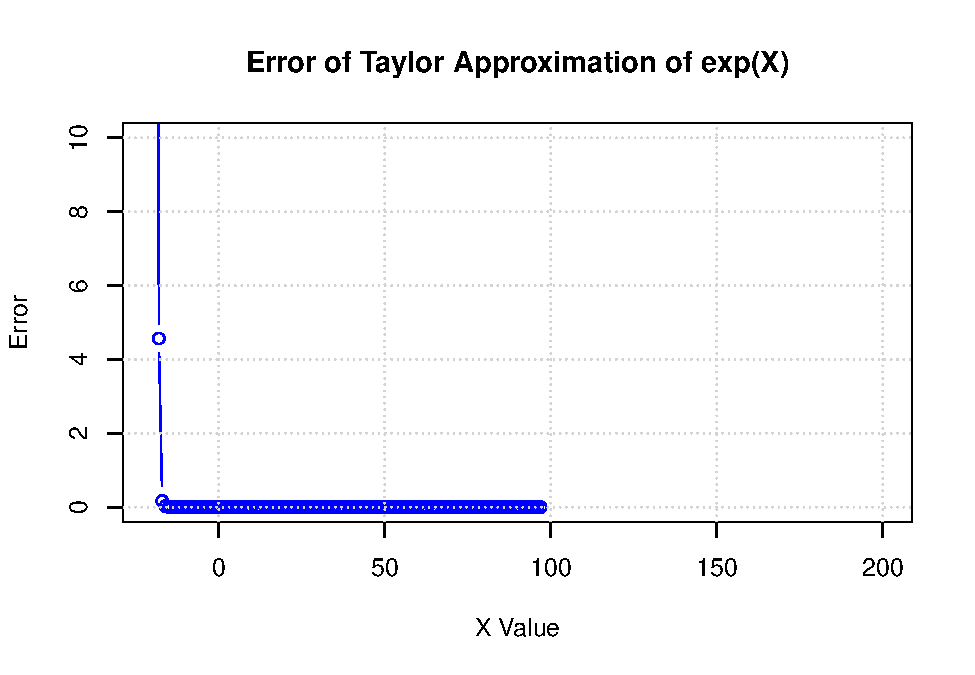
\includegraphics[keepaspectratio]{H1_files/figure-latex/unnamed-chunk-9-1.pdf}}

We notice that for lower values, MAPE increases starting approximately
from \(-10\).\\
For values of \(X\) higher than \(100\), MAPE is absent as the
approximation of the exponent is probably equal to \(\infty\).

Let us check:

\begin{Shaded}
\begin{Highlighting}[]
\NormalTok{X }\OtherTok{\textless{}{-}} \DecValTok{101}

\FunctionTok{cat}\NormalTok{(}\StringTok{"Our function:"}\NormalTok{, }\FunctionTok{calculate\_exp}\NormalTok{(X), }\StringTok{"}\SpecialCharTok{\textbackslash{}n}\StringTok{"}\NormalTok{)}
\end{Highlighting}
\end{Shaded}

\begin{verbatim}
## Our function: Inf
\end{verbatim}

\begin{Shaded}
\begin{Highlighting}[]
\FunctionTok{cat}\NormalTok{(}\StringTok{"R actual function"}\NormalTok{, }\FunctionTok{exp}\NormalTok{(X), }\StringTok{"}\SpecialCharTok{\textbackslash{}n}\StringTok{"}\NormalTok{)}
\end{Highlighting}
\end{Shaded}

\begin{verbatim}
## R actual function 7.30706e+43
\end{verbatim}

\begin{Shaded}
\begin{Highlighting}[]
\NormalTok{X }\OtherTok{\textless{}{-}} \SpecialCharTok{{-}}\DecValTok{20}

\FunctionTok{cat}\NormalTok{(}\StringTok{"Our function:"}\NormalTok{, }\FunctionTok{calculate\_exp}\NormalTok{(X), }\StringTok{"}\SpecialCharTok{\textbackslash{}n}\StringTok{"}\NormalTok{)}
\end{Highlighting}
\end{Shaded}

\begin{verbatim}
## Our function: 4.992704e-09
\end{verbatim}

\begin{Shaded}
\begin{Highlighting}[]
\FunctionTok{cat}\NormalTok{(}\StringTok{"R actual function"}\NormalTok{, }\FunctionTok{exp}\NormalTok{(X), }\StringTok{"}\SpecialCharTok{\textbackslash{}n}\StringTok{"}\NormalTok{)}
\end{Highlighting}
\end{Shaded}

\begin{verbatim}
## R actual function 2.061154e-09
\end{verbatim}

Indeed, either our approximations are too far from the actual values of
the function, or our approximations are equal to infinity.

\subsection{(iii)}\label{iii}

Let us suggest a modification how to fix the numerical instability. We
use the following property:

\[
e^{x} = \left(e^{x/n}\right)^n
\]

We implement it in our updated function as a wrapper:

\begin{Shaded}
\begin{Highlighting}[]
\NormalTok{calculate\_exp\_2 }\OtherTok{\textless{}{-}} \ControlFlowTok{function}\NormalTok{(x, }\AttributeTok{n =} \DecValTok{10}\NormalTok{) \{}
\NormalTok{    x\_n }\OtherTok{\textless{}{-}}\NormalTok{ x }\SpecialCharTok{/}\NormalTok{ n}
\NormalTok{    result }\OtherTok{\textless{}{-}} \FunctionTok{calculate\_exp}\NormalTok{(x\_n)}\SpecialCharTok{\^{}}\NormalTok{n}
    \FunctionTok{return}\NormalTok{(result)}
\NormalTok{\}}
\end{Highlighting}
\end{Shaded}

Let's first check it for single values:

\begin{Shaded}
\begin{Highlighting}[]
\NormalTok{X }\OtherTok{\textless{}{-}} \SpecialCharTok{{-}}\DecValTok{20}

\FunctionTok{cat}\NormalTok{(}\StringTok{"Our function:"}\NormalTok{, }\FunctionTok{calculate\_exp\_2}\NormalTok{(X), }\StringTok{"}\SpecialCharTok{\textbackslash{}n}\StringTok{"}\NormalTok{)}
\end{Highlighting}
\end{Shaded}

\begin{verbatim}
## Our function: 2.061154e-09
\end{verbatim}

\begin{Shaded}
\begin{Highlighting}[]
\FunctionTok{cat}\NormalTok{(}\StringTok{"R actual function"}\NormalTok{, }\FunctionTok{exp}\NormalTok{(X), }\StringTok{"}\SpecialCharTok{\textbackslash{}n}\StringTok{"}\NormalTok{)}
\end{Highlighting}
\end{Shaded}

\begin{verbatim}
## R actual function 2.061154e-09
\end{verbatim}

\begin{Shaded}
\begin{Highlighting}[]
\NormalTok{X }\OtherTok{\textless{}{-}} \DecValTok{101}

\FunctionTok{cat}\NormalTok{(}\StringTok{"Our function:"}\NormalTok{, }\FunctionTok{calculate\_exp\_2}\NormalTok{(X), }\StringTok{"}\SpecialCharTok{\textbackslash{}n}\StringTok{"}\NormalTok{)}
\end{Highlighting}
\end{Shaded}

\begin{verbatim}
## Our function: 7.30706e+43
\end{verbatim}

\begin{Shaded}
\begin{Highlighting}[]
\FunctionTok{cat}\NormalTok{(}\StringTok{"R actual function"}\NormalTok{, }\FunctionTok{exp}\NormalTok{(X), }\StringTok{"}\SpecialCharTok{\textbackslash{}n}\StringTok{"}\NormalTok{)}
\end{Highlighting}
\end{Shaded}

\begin{verbatim}
## R actual function 7.30706e+43
\end{verbatim}

And now for our range:

\begin{Shaded}
\begin{Highlighting}[]
\NormalTok{X\_values }\OtherTok{\textless{}{-}} \FunctionTok{seq}\NormalTok{(}\SpecialCharTok{{-}}\DecValTok{20}\NormalTok{, }\DecValTok{200}\NormalTok{, }\AttributeTok{by=}\DecValTok{1}\NormalTok{)}
\NormalTok{errors }\OtherTok{\textless{}{-}} \FunctionTok{numeric}\NormalTok{(}\FunctionTok{length}\NormalTok{(X\_values)) }

\ControlFlowTok{for}\NormalTok{ (i }\ControlFlowTok{in} \FunctionTok{seq\_along}\NormalTok{(X\_values)) \{}
\NormalTok{  X }\OtherTok{\textless{}{-}}\NormalTok{ X\_values[i]}
  
  
\NormalTok{ mape }\OtherTok{\textless{}{-}} \FunctionTok{mean}\NormalTok{(}\FunctionTok{abs}\NormalTok{((}\FunctionTok{exp}\NormalTok{(X) }\SpecialCharTok{{-}} \FunctionTok{calculate\_exp\_2}\NormalTok{(X)) }\SpecialCharTok{/} \FunctionTok{exp}\NormalTok{(X))) }\SpecialCharTok{*} \DecValTok{100}

  
  
\NormalTok{  errors[i] }\OtherTok{\textless{}{-}}\NormalTok{ mape  }
\NormalTok{\}}

\CommentTok{\# plotting}

\FunctionTok{plot}\NormalTok{(X\_values, errors, }\AttributeTok{type =} \StringTok{"b"}\NormalTok{, }\AttributeTok{col =} \StringTok{"blue"}\NormalTok{,}
     \AttributeTok{xlab =} \StringTok{"X Value"}\NormalTok{, }\AttributeTok{ylab =} \StringTok{"Error"}\NormalTok{,}
     \AttributeTok{main =} \StringTok{"Error of Taylor Approximation of exp(X)"}\NormalTok{,}
     \AttributeTok{ylim =} \FunctionTok{c}\NormalTok{(}\DecValTok{0}\NormalTok{, }\DecValTok{10}\NormalTok{))  }\CommentTok{\# Adjust these limits as needed for your data}
\FunctionTok{grid}\NormalTok{()}
\end{Highlighting}
\end{Shaded}

\pandocbounded{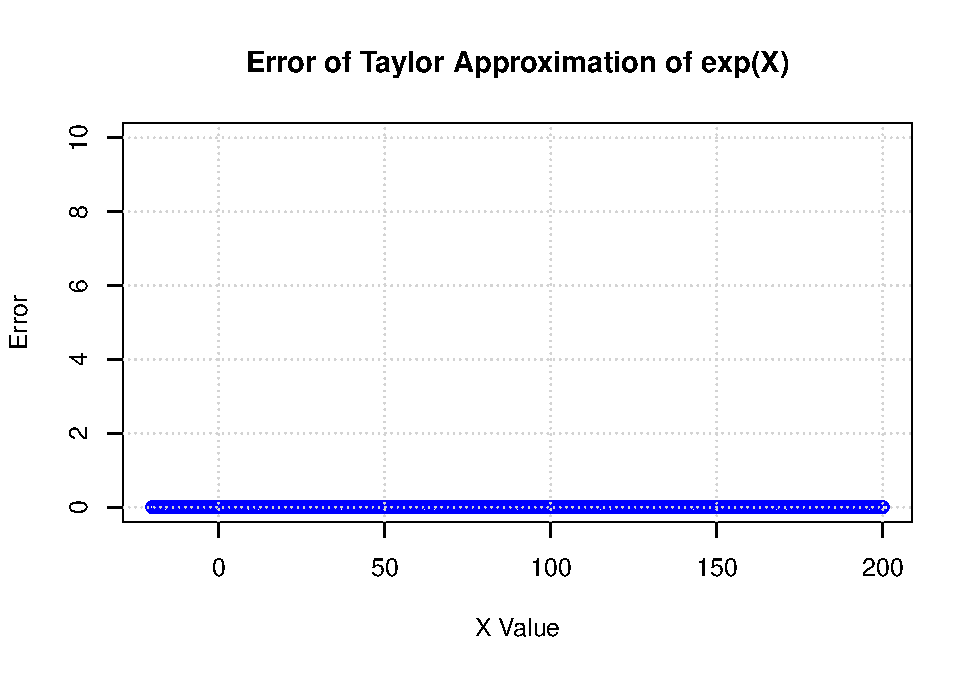
\includegraphics[keepaspectratio]{H1_files/figure-latex/unnamed-chunk-15-1.pdf}}

All looks good!

\section{Exercise 4}\label{exercise-4}

We want to calculate

\$\$

\frac{\sqrt{1 +x}-1}{x}

\$\$

\subsection{i Determine the values of R for x =1, 10\^{}-4,
10\^{}-32}\label{i-determine-the-values-of-r-for-x-1-10-4-10-32}

\begin{Shaded}
\begin{Highlighting}[]
\NormalTok{function\_x }\OtherTok{\textless{}{-}} \ControlFlowTok{function}\NormalTok{(x) \{}
  \FunctionTok{return}\NormalTok{((}\FunctionTok{sqrt}\NormalTok{(}\DecValTok{1} \SpecialCharTok{+}\NormalTok{ x) }\SpecialCharTok{{-}} \DecValTok{1}\NormalTok{) }\SpecialCharTok{/}\NormalTok{ x)}
\NormalTok{\}}

\NormalTok{function\_x\_rationalisation }\OtherTok{\textless{}{-}} \ControlFlowTok{function}\NormalTok{(x) \{}
  \FunctionTok{return}\NormalTok{(}\DecValTok{1} \SpecialCharTok{/}\NormalTok{ (}\FunctionTok{sqrt}\NormalTok{(}\DecValTok{1} \SpecialCharTok{+}\NormalTok{ x) }\SpecialCharTok{+} \DecValTok{1}\NormalTok{))}
\NormalTok{\}}


\FunctionTok{function\_x}\NormalTok{(}\DecValTok{1}\NormalTok{)}
\end{Highlighting}
\end{Shaded}

\begin{verbatim}
## [1] 0.4142136
\end{verbatim}

\begin{Shaded}
\begin{Highlighting}[]
\FunctionTok{function\_x}\NormalTok{(}\DecValTok{10}\SpecialCharTok{\^{}}\NormalTok{(}\SpecialCharTok{{-}}\DecValTok{4}\NormalTok{))}
\end{Highlighting}
\end{Shaded}

\begin{verbatim}
## [1] 0.4999875
\end{verbatim}

\begin{Shaded}
\begin{Highlighting}[]
\FunctionTok{function\_x}\NormalTok{(}\DecValTok{10}\SpecialCharTok{\^{}}\NormalTok{(}\SpecialCharTok{{-}}\DecValTok{32}\NormalTok{))}
\end{Highlighting}
\end{Shaded}

\begin{verbatim}
## [1] 0
\end{verbatim}

\subsection{\texorpdfstring{ii, iii Use the Taylor series of
\[\sqrt{1+x}\] to approximate the result for small values of x. And
Implement an approximate calculation of the result based on the Taylor
series.}{ii, iii Use the Taylor series of \textbackslash sqrt\{1+x\} to approximate the result for small values of x. And Implement an approximate calculation of the result based on the Taylor series.}}\label{ii-iii-use-the-taylor-series-of-sqrt1x-to-approximate-the-result-for-small-values-of-x.-and-implement-an-approximate-calculation-of-the-result-based-on-the-taylor-series.}

\begin{Shaded}
\begin{Highlighting}[]
\NormalTok{taylor\_expansion\_at\_zero }\OtherTok{\textless{}{-}} \ControlFlowTok{function}\NormalTok{(y) \{}
  \FunctionTok{return}\NormalTok{(}\DecValTok{1} \SpecialCharTok{+}\NormalTok{ y }\SpecialCharTok{/} \DecValTok{2} \SpecialCharTok{{-}}\NormalTok{ y}\SpecialCharTok{\^{}}\DecValTok{2} \SpecialCharTok{/} \DecValTok{8} \SpecialCharTok{+}\NormalTok{ y}\SpecialCharTok{\^{}}\DecValTok{3} \SpecialCharTok{/} \DecValTok{16} \SpecialCharTok{{-}} \DecValTok{5} \SpecialCharTok{*}\NormalTok{ y}\SpecialCharTok{\^{}}\DecValTok{4} \SpecialCharTok{/} \DecValTok{128} \SpecialCharTok{+} \DecValTok{7} \SpecialCharTok{*}\NormalTok{ y}\SpecialCharTok{\^{}}\DecValTok{5} \SpecialCharTok{/} \DecValTok{256}\NormalTok{)}
\NormalTok{\}}

\NormalTok{approximation\_result\_function\_x\_at\_zero }\OtherTok{\textless{}{-}} \ControlFlowTok{function}\NormalTok{(x) \{}
  \FunctionTok{return}\NormalTok{((}\FunctionTok{taylor\_expansion\_at\_zero}\NormalTok{(x) }\SpecialCharTok{{-}} \DecValTok{1}\NormalTok{) }\SpecialCharTok{/}\NormalTok{ x)}
\NormalTok{\}}

\FunctionTok{approximation\_result\_function\_x\_at\_zero}\NormalTok{(}\DecValTok{1}\NormalTok{)}
\end{Highlighting}
\end{Shaded}

\begin{verbatim}
## [1] 0.4257812
\end{verbatim}

\begin{Shaded}
\begin{Highlighting}[]
\FunctionTok{approximation\_result\_function\_x\_at\_zero}\NormalTok{(}\DecValTok{10}\SpecialCharTok{\^{}}\NormalTok{(}\SpecialCharTok{{-}}\DecValTok{4}\NormalTok{))}
\end{Highlighting}
\end{Shaded}

\begin{verbatim}
## [1] 0.4999875
\end{verbatim}

\begin{Shaded}
\begin{Highlighting}[]
\FunctionTok{approximation\_result\_function\_x\_at\_zero}\NormalTok{(}\DecValTok{10}\SpecialCharTok{\^{}}\NormalTok{(}\SpecialCharTok{{-}}\DecValTok{32}\NormalTok{))}
\end{Highlighting}
\end{Shaded}

\begin{verbatim}
## [1] 0
\end{verbatim}

\begin{Shaded}
\begin{Highlighting}[]
\CommentTok{\# Create a loop that stores the results of a multiplication in a vector}
\NormalTok{multiplication\_results\_negative }\OtherTok{\textless{}{-}} \FunctionTok{numeric}\NormalTok{(}\DecValTok{100}\NormalTok{)}
\NormalTok{multiplication\_results\_positive }\OtherTok{\textless{}{-}} \FunctionTok{numeric}\NormalTok{(}\DecValTok{100}\NormalTok{)}

\ControlFlowTok{for}\NormalTok{ (i }\ControlFlowTok{in} \FunctionTok{seq\_len}\NormalTok{(}\DecValTok{200}\NormalTok{)) \{}
\NormalTok{  multiplication\_results\_negative[i] }\OtherTok{\textless{}{-}}\NormalTok{ .Machine}\SpecialCharTok{$}\NormalTok{double.eps}\SpecialCharTok{*}\NormalTok{i }\SpecialCharTok{+} \DecValTok{0}
\NormalTok{  multiplication\_results\_positive[i] }\OtherTok{\textless{}{-}} \SpecialCharTok{{-}}\NormalTok{.Machine}\SpecialCharTok{$}\NormalTok{double.eps}\SpecialCharTok{*}\NormalTok{i }\SpecialCharTok{+} \DecValTok{0}
\NormalTok{\}}

\NormalTok{combined\_results }\OtherTok{\textless{}{-}} \FunctionTok{c}\NormalTok{(multiplication\_results\_negative, multiplication\_results\_positive)}
\NormalTok{sorted\_results }\OtherTok{\textless{}{-}} \FunctionTok{sort}\NormalTok{(combined\_results)}
\end{Highlighting}
\end{Shaded}

\subsection{Compare the results for the two different calculations
visually with a focus on small values of x. Explain what the problem
is.}\label{compare-the-results-for-the-two-different-calculations-visually-with-a-focus-on-small-values-of-x.-explain-what-the-problem-is.}

\begin{Shaded}
\begin{Highlighting}[]
\NormalTok{function\_x\_values }\OtherTok{\textless{}{-}} \FunctionTok{sapply}\NormalTok{(sorted\_results, function\_x)}
\NormalTok{approximation\_values }\OtherTok{\textless{}{-}} \FunctionTok{sapply}\NormalTok{(sorted\_results, approximation\_result\_function\_x\_at\_zero)}
\NormalTok{function\_x\_rationalisation\_values }\OtherTok{\textless{}{-}} \FunctionTok{sapply}\NormalTok{(sorted\_results, function\_x\_rationalisation)}

\FunctionTok{plot}\NormalTok{(sorted\_results, function\_x\_values, }\AttributeTok{type =} \StringTok{"l"}\NormalTok{, }\AttributeTok{col =} \StringTok{"blue"}\NormalTok{, }\AttributeTok{ylim =} \FunctionTok{range}\NormalTok{(}\FunctionTok{c}\NormalTok{(function\_x\_values, approximation\_values)), }\AttributeTok{ylab =} \StringTok{"Values"}\NormalTok{, }\AttributeTok{xlab =} \StringTok{"x"}\NormalTok{, }\AttributeTok{main =} \StringTok{"Comparison of function\_x and its Taylor Approximation"}\NormalTok{)}
\FunctionTok{lines}\NormalTok{(sorted\_results, approximation\_values, }\AttributeTok{col =} \StringTok{"red"}\NormalTok{)}
\FunctionTok{lines}\NormalTok{(sorted\_results, function\_x\_rationalisation\_values, }\AttributeTok{col =} \StringTok{"green"}\NormalTok{)}
\FunctionTok{legend}\NormalTok{(}\StringTok{"topright"}\NormalTok{, }\AttributeTok{legend =} \FunctionTok{c}\NormalTok{(}\StringTok{"function\_x"}\NormalTok{, }\StringTok{"Taylor Expansion"}\NormalTok{, }\StringTok{"Function\_x\_rationalisation"}\NormalTok{), }\AttributeTok{col =} \FunctionTok{c}\NormalTok{(}\StringTok{"blue"}\NormalTok{, }\StringTok{"red"}\NormalTok{,}\StringTok{"green"}\NormalTok{), }\AttributeTok{lty =} \DecValTok{1}\NormalTok{)}
\end{Highlighting}
\end{Shaded}

\pandocbounded{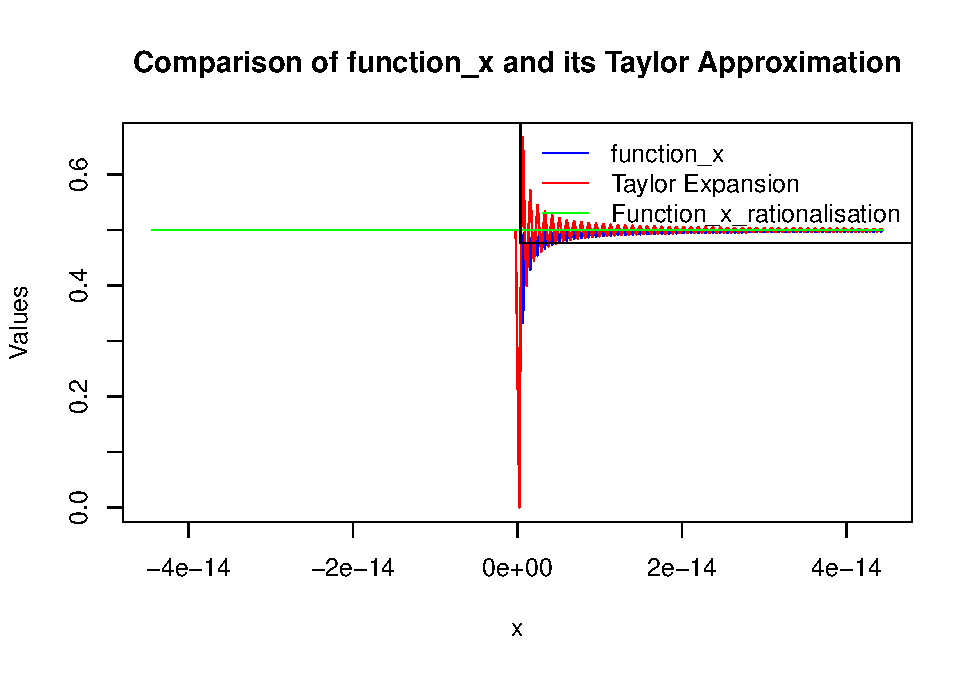
\includegraphics[keepaspectratio]{H1_files/figure-latex/unnamed-chunk-18-1.pdf}}

\begin{Shaded}
\begin{Highlighting}[]
\CommentTok{\# With greater values of around o}
\NormalTok{increment\_values }\OtherTok{\textless{}{-}} \FunctionTok{seq}\NormalTok{(}\SpecialCharTok{{-}}\FloatTok{0.0005}\NormalTok{, }\FloatTok{0.0005}\NormalTok{, }\AttributeTok{length.out =} \DecValTok{1000}\NormalTok{)}

\CommentTok{\# Calculate function values for the new vector}
\NormalTok{function\_x\_increment\_values }\OtherTok{\textless{}{-}} \FunctionTok{sapply}\NormalTok{(increment\_values, function\_x)}
\NormalTok{approximation\_increment\_values }\OtherTok{\textless{}{-}} \FunctionTok{sapply}\NormalTok{(increment\_values, approximation\_result\_function\_x\_at\_zero)}
\NormalTok{function\_x\_rationalisation\_increment\_values }\OtherTok{\textless{}{-}} \FunctionTok{sapply}\NormalTok{(increment\_values, function\_x\_rationalisation)}

\CommentTok{\# Plot the new values}
\FunctionTok{plot}\NormalTok{(increment\_values, function\_x\_increment\_values, }\AttributeTok{type =} \StringTok{"l"}\NormalTok{, }\AttributeTok{col =} \StringTok{"blue"}\NormalTok{, }\AttributeTok{ylim =} \FunctionTok{range}\NormalTok{(}\FunctionTok{c}\NormalTok{(function\_x\_increment\_values, approximation\_increment\_values)), }\AttributeTok{ylab =} \StringTok{"Values"}\NormalTok{, }\AttributeTok{xlab =} \StringTok{"x"}\NormalTok{, }\AttributeTok{main =} \StringTok{"Comparison of function\_x and its Taylor Approximation"}\NormalTok{)}
\FunctionTok{lines}\NormalTok{(increment\_values, approximation\_increment\_values, }\AttributeTok{col =} \StringTok{"red"}\NormalTok{)}
\FunctionTok{lines}\NormalTok{(increment\_values, function\_x\_rationalisation\_increment\_values, }\AttributeTok{col =} \StringTok{"green"}\NormalTok{)}
\FunctionTok{legend}\NormalTok{(}\StringTok{"topright"}\NormalTok{, }\AttributeTok{legend =} \FunctionTok{c}\NormalTok{(}\StringTok{"function\_x"}\NormalTok{, }\StringTok{"Taylor Expansion"}\NormalTok{, }\StringTok{"Function\_x\_rationalisation"}\NormalTok{), }\AttributeTok{col =} \FunctionTok{c}\NormalTok{(}\StringTok{"blue"}\NormalTok{, }\StringTok{"red"}\NormalTok{, }\StringTok{"green"}\NormalTok{), }\AttributeTok{lty =} \DecValTok{1}\NormalTok{)}
\end{Highlighting}
\end{Shaded}

\pandocbounded{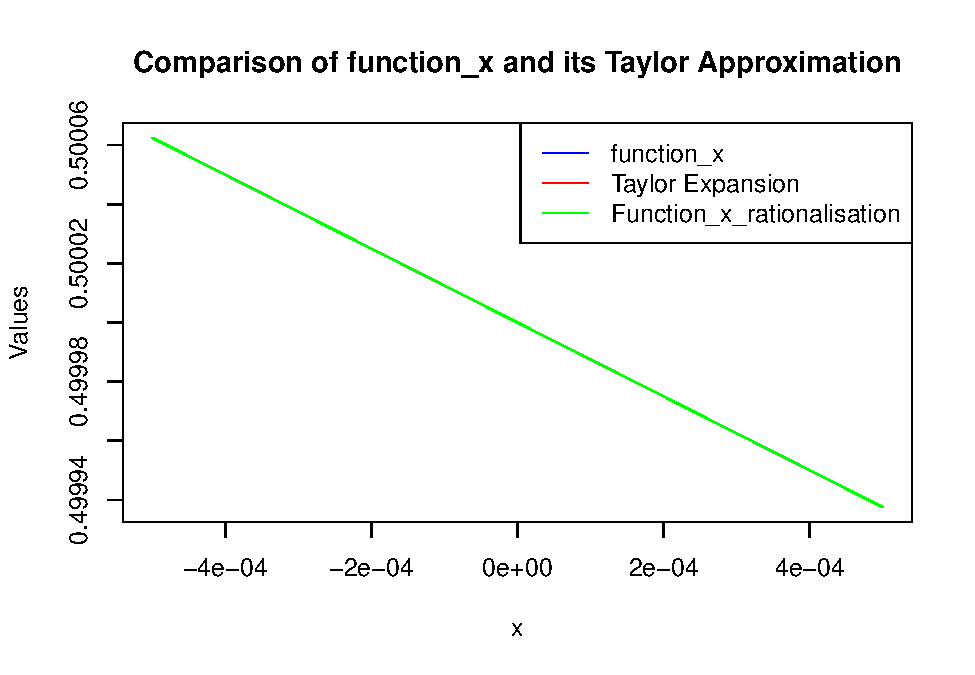
\includegraphics[keepaspectratio]{H1_files/figure-latex/unnamed-chunk-18-2.pdf}}

\begin{Shaded}
\begin{Highlighting}[]
\FunctionTok{print}\NormalTok{(function\_x\_increment\_values[}\DecValTok{1}\NormalTok{])}
\end{Highlighting}
\end{Shaded}

\begin{verbatim}
## [1] 0.5000625
\end{verbatim}

\begin{Shaded}
\begin{Highlighting}[]
\FunctionTok{print}\NormalTok{(approximation\_increment\_values[}\DecValTok{1}\NormalTok{])}
\end{Highlighting}
\end{Shaded}

\begin{verbatim}
## [1] 0.5000625
\end{verbatim}

\begin{Shaded}
\begin{Highlighting}[]
\FunctionTok{print}\NormalTok{(function\_x\_rationalisation\_increment\_values[}\DecValTok{1}\NormalTok{])}
\end{Highlighting}
\end{Shaded}

\begin{verbatim}
## [1] 0.5000625
\end{verbatim}

Answer: As shown in the first graph, the divergences between the values
of the taylor approximation, and the function in its two forms differ
when the values of zero are very small of the order of
.Machine\(double.eps that
represents the minimal difference stored in doubles so that 1 + .Machine\)double.eps
is recognized as different than 1. According to what we saw in class we
can think on two possible answers. Similar to computing the mean either
through the sum of squares of deviations or as the differences between
the mean of the squared values and the squared value of the mean, it may
be R uses different process to solve (sqrt) and polynomial fractions
that yield different results for very small values of x. It can be also
that the taylor approximation is not accurate enough for very small
values of x.

\section{Exercise 5}\label{exercise-5}

\begin{Shaded}
\begin{Highlighting}[]
\FunctionTok{data}\NormalTok{(}\StringTok{"KNex"}\NormalTok{, }\AttributeTok{package =} \StringTok{"Matrix"}\NormalTok{)}
\NormalTok{X }\OtherTok{\textless{}{-}} \FunctionTok{as.matrix}\NormalTok{(KNex}\SpecialCharTok{$}\NormalTok{mm)}
\NormalTok{Y }\OtherTok{\textless{}{-}}\NormalTok{ KNex}\SpecialCharTok{$}\NormalTok{y}

\CommentTok{\# It may be more accurate ways to compute the type of execution.}
\NormalTok{start\_time }\OtherTok{\textless{}{-}} \FunctionTok{Sys.time}\NormalTok{()}
\NormalTok{fit }\OtherTok{\textless{}{-}} \FunctionTok{lm.fit}\NormalTok{(X, Y)}
\NormalTok{end\_time }\OtherTok{\textless{}{-}} \FunctionTok{Sys.time}\NormalTok{()}
\NormalTok{execution\_time\_lmfit }\OtherTok{\textless{}{-}}\NormalTok{ end\_time }\SpecialCharTok{{-}}\NormalTok{ start\_time}
\FunctionTok{print}\NormalTok{(}\FunctionTok{paste}\NormalTok{(}\StringTok{"Execution time:"}\NormalTok{, execution\_time\_lmfit ))}
\end{Highlighting}
\end{Shaded}

\begin{verbatim}
## [1] "Execution time: 0.483719825744629"
\end{verbatim}

\begin{Shaded}
\begin{Highlighting}[]
\CommentTok{\# Formula of Least Square estimator B = (X\^{}T X)\^{}{-}1 X\^{}T Y}
\CommentTok{\# Let us try to find this (X\^{}T X)\^{}{-}1 part with }

\DocumentationTok{\#\#\#\#\#\#\#\#\#\#\#\#\#\#\#\#\#\#\#\#\#\#\#\#\#\#\#\#\#\#\#\#\#\#\#\#\#\#\#\#\#\#\#\#\#\#\#\#\#\#\#}
\DocumentationTok{\#\#\# Cholesky decomposition}
\DocumentationTok{\#\#\#\#\#\#\#\#\#\#\#\#\#\#\#\#\#\#\#\#\#\#\#\#\#\#\#\#\#\#\#\#\#\#\#\#\#\#\#\#\#\#\#\#\#\#\#\#\#\#\#}
\CommentTok{\# We find the product of the matrix X\^{}TX (This matrix is symetric)}
\CommentTok{\# Crossprod makes it so that it computes only the lower triangular product, it does then only }
\CommentTok{\# half of the work, by computing only the upper triangular part of the matrix.}


\NormalTok{R }\OtherTok{\textless{}{-}} \FunctionTok{chol}\NormalTok{(}\FunctionTok{crossprod}\NormalTok{(X))}

\CommentTok{\# Using Solve to find the inverse of both matrix and to multiply the right upper triangular matrix}

\NormalTok{start\_time }\OtherTok{\textless{}{-}} \FunctionTok{Sys.time}\NormalTok{()}
\NormalTok{chol\_betas }\OtherTok{\textless{}{-}} \FunctionTok{backsolve}\NormalTok{(R, }\FunctionTok{forwardsolve}\NormalTok{(R, }\FunctionTok{crossprod}\NormalTok{(X, Y), }\AttributeTok{upper.tri =} \ConstantTok{TRUE}\NormalTok{, }\AttributeTok{transpose =} \ConstantTok{TRUE}\NormalTok{))}
\NormalTok{end\_time }\OtherTok{\textless{}{-}} \FunctionTok{Sys.time}\NormalTok{()}
\NormalTok{execution\_time\_chol }\OtherTok{\textless{}{-}}\NormalTok{ end\_time }\SpecialCharTok{{-}}\NormalTok{ start\_time}
\FunctionTok{print}\NormalTok{(}\FunctionTok{paste}\NormalTok{(}\StringTok{"Execution time:"}\NormalTok{, execution\_time\_chol))}
\end{Highlighting}
\end{Shaded}

\begin{verbatim}
## [1] "Execution time: 0.00437688827514648"
\end{verbatim}

\begin{Shaded}
\begin{Highlighting}[]
\DocumentationTok{\#\#\#\#\#\#\#\#\#\#\#\#\#\#\#\#\#\#\#\#\#\#\#\#\#\#\#\#\#\#\#\#\#\#\#\#\#\#\#\#\#\#\#\#\#\#\#\#\#\#\#}
\DocumentationTok{\#\#\# QR decomposition}
\DocumentationTok{\#\#\#\#\#\#\#\#\#\#\#\#\#\#\#\#\#\#\#\#\#\#\#\#\#\#\#\#\#\#\#\#\#\#\#\#\#\#\#\#\#\#\#\#\#\#\#\#\#\#\#}
\NormalTok{QR }\OtherTok{\textless{}{-}} \FunctionTok{qr}\NormalTok{(X)}
\NormalTok{qr\_betas }\OtherTok{\textless{}{-}} \FunctionTok{backsolve}\NormalTok{(}\FunctionTok{qr.R}\NormalTok{(QR), }\FunctionTok{crossprod}\NormalTok{(}\FunctionTok{qr.Q}\NormalTok{(QR), Y))}
\FunctionTok{solve}\NormalTok{(QR, Y)}
\end{Highlighting}
\end{Shaded}

\begin{verbatim}
##   [1]  8.233613e+02  3.401156e+02  4.729760e+02  3.493175e+02  1.875595e+02
##   [6]  1.590518e+02 -5.488358e+01  4.976512e+02  5.747553e+02  5.844035e+02
##  [11]  4.433759e+02  4.598322e+02  4.377678e+02  4.718594e+02  2.518818e+02
##  [16]  3.870411e+02  3.069063e+02  4.240379e+02  2.789121e+02  2.792760e+02
##  [21]  1.343340e+02  1.751695e+02  1.964427e+02  1.840951e+02  1.475290e+02
##  [26]  1.251323e+02  2.065104e+02  2.069963e+02  2.292703e+02  1.559251e+02
##  [31]  1.519143e+02  7.014589e+01  3.905758e+01  8.530887e+01  1.543696e+02
##  [36]  2.057099e+02  2.319248e+02  9.776988e+02  7.925844e+02  8.881473e+02
##  [41]  2.353893e+02  4.792704e+02  3.281097e+02  4.429996e+02  2.186452e+02
##  [46]  1.563899e+02  2.958011e+02  3.844060e+02  4.234291e+02  5.509931e+02
##  [51]  6.758963e+02  8.035716e+02  6.621915e+02  6.011474e+02  3.680682e+02
##  [56]  5.663948e+02  3.949569e+02  2.959356e+02  4.336161e+02  3.104814e+02
##  [61]  2.953505e+02  4.065316e+02  3.047238e+02  3.895511e+02  3.644747e+02
##  [66]  4.792018e+02  4.739014e+02  3.893197e+02  4.114851e+02  3.262520e+02
##  [71]  3.521532e+02  2.109392e+02  4.867653e+01  2.854132e+02  1.665921e+02
##  [76]  2.157594e+02  2.942907e+02  1.275330e+03  4.377361e+02  1.141416e+03
##  [81]  6.743610e+02  5.796302e+02  8.075738e+02  3.486425e+02  3.109191e+02
##  [86]  3.235872e+02  3.140781e+02  2.645482e+02  2.515995e+02  2.668293e+01
##  [91]  1.040061e+02  4.310320e+02  6.200368e+02  6.680256e+02  6.720507e+02
##  [96]  2.009096e+02  1.034493e+02  1.984021e+02  1.733915e+02  1.181538e+02
## [101]  2.292999e+02  1.520113e+02  1.810291e+02  8.822708e+01  7.352156e+01
## [106]  7.937319e+02  9.772659e+02  6.511196e+02  5.466706e+02  4.611334e+02
## [111]  3.752323e+02  6.064726e+02  1.147064e+03  8.704502e+02  7.476932e+02
## [116]  1.567143e+03  1.109384e+03  1.234439e+03  3.679044e+02  1.602590e+03
## [121]  6.098344e+02  1.056413e+03  1.026361e+03  1.153084e+03  9.729797e+02
## [126]  8.503641e+02  1.177652e+03  1.540202e+03  4.386716e+02  9.095268e+02
## [131]  5.232499e+02  4.384315e+02  5.248368e+02  3.540961e+02  9.983145e+01
## [136]  1.414522e+02  3.041497e+02  4.789437e+02  7.907425e+02  1.280902e+03
## [141]  7.796757e+02  1.186552e+03  9.128162e+02  5.312751e+02  8.118134e+02
## [146]  4.574875e+02  5.215645e+02  1.584941e+03  1.316831e+03  9.139825e+02
## [151]  1.216854e+03  4.147569e+02  1.186420e+03  7.411721e+02  1.027085e+03
## [156]  1.075455e+03  5.817779e+02  5.458053e+02  1.212961e+03  1.540449e+03
## [161]  1.236405e+03  1.851630e+03  9.306336e+02  1.372048e+03  1.362646e+03
## [166]  1.813367e+03  1.286375e+03  1.234847e+03  1.149278e+03  8.808191e+02
## [171]  5.961477e+02  1.694015e+03  1.596274e+03  1.444483e+03  2.077174e+03
## [176]  1.324911e+03  1.260746e+03  2.005284e+03  9.712938e+02  8.840197e+02
## [181]  1.402016e+03  1.214940e+03  1.240159e+03  9.550797e+02  1.063108e+03
## [186]  1.199806e+03  1.308148e+03  5.451265e+02  1.181646e+03  6.112288e+02
## [191]  1.264504e+03  1.603506e+03  5.882915e+02  1.501174e+03  1.119449e+03
## [196]  4.965155e+02  1.197639e+03  1.606044e+03  1.548944e+03  1.697874e+03
## [201]  1.882957e+03  1.071097e+03  8.124339e+02  1.149240e+03  9.166338e+02
## [206]  1.336850e+03  1.205886e+03  1.723131e+03  1.363899e+03  1.328714e+03
## [211]  1.010324e+03  3.484667e+02  9.050154e+02  9.050259e+02  4.532011e+02
## [216]  1.222204e+02  1.273822e+03  5.744192e+02  6.686459e+01  1.649687e+02
## [221]  2.399577e+02  7.774156e+01  7.418588e+02  6.931921e+02  6.202376e+02
## [226]  4.110494e+02  4.989011e+02  6.085244e+02  5.216533e+02  7.558672e+02
## [231]  6.974754e+02  9.130571e+02  8.533190e+02  9.546704e+02  1.003512e+03
## [236]  3.718109e+02  5.194766e+02  6.615869e+02  5.448740e+02  6.171181e+02
## [241]  5.679168e+02  6.594026e+02  5.743472e+02  6.086175e+02  6.415078e+02
## [246]  6.260161e+02  4.611107e+02  4.867161e+02  4.907317e+02  5.547498e+02
## [251]  4.522325e+02  2.406329e+02  7.264263e+02  1.087639e+03 -5.977955e+02
## [256]  3.021057e+02  1.141091e+02 -3.285763e+02 -2.645895e+02 -9.350325e+01
## [261]  8.480110e+01 -4.075880e+02 -4.906305e+02 -2.346200e+02 -3.516962e+02
## [266] -2.620967e+02 -2.183761e+02 -2.931662e+02 -1.012603e+02 -1.418004e+02
## [271] -6.184407e+01  5.222349e+01 -6.411881e+00 -9.958820e+01 -8.468244e+01
## [276] -2.985685e+01  2.176049e+00  2.432122e+00  5.447453e+01 -6.728951e+02
## [281] -3.930567e+02 -2.133295e+02 -2.611774e+02 -1.294373e+02 -1.451921e+02
## [286] -1.728689e+02 -3.641853e+02 -3.458473e+02 -3.454447e+02 -5.180689e+02
## [291] -3.862287e+02 -3.861784e+02 -4.574517e+02 -5.558451e+02 -4.695612e+02
## [296] -5.180875e+02 -4.881248e+02 -1.068728e+02 -1.921435e+01 -6.810688e+01
## [301] -1.374622e+02 -2.399132e+02 -7.669983e+02 -7.796899e+02 -3.011046e+02
## [306] -3.115064e+02 -1.894849e+02 -1.159407e+02  1.281760e+01  1.096485e+01
## [311]  7.315653e+01 -1.726737e+01 -1.035809e+02 -2.638569e+02 -2.643346e+02
## [316] -4.596594e+01 -3.479583e+01 -2.596215e+01 -1.479574e+02 -6.500528e+02
## [321] -4.910204e+02 -4.220341e+02 -4.129418e+02 -3.376096e+02 -1.413364e+02
## [326] -4.620433e+02 -3.772590e+02 -5.899099e+02 -7.454992e+02 -4.560824e+02
## [331] -5.890350e+02 -5.893740e+02 -3.980780e+02 -5.141775e+02 -5.993717e+02
## [336] -1.028976e+03 -1.139867e+03 -6.884250e+02 -3.896642e+02 -5.064374e+02
## [341] -3.033843e+02 -2.818138e+02 -9.205401e+01 -2.282751e+02 -8.895736e+01
## [346] -1.619924e+02 -2.307575e+02 -3.658412e+02 -2.333038e+02 -3.596782e+02
## [351] -2.922361e+02 -3.922122e+02 -6.113374e+02 -8.086072e+02 -5.711833e+02
## [356] -6.494190e+02 -9.423636e+02 -5.152641e+02 -8.230401e+02 -6.839862e+02
## [361] -7.121826e+02 -1.325016e+03 -7.963237e+02 -1.125432e+03 -1.101174e+03
## [366] -1.766877e+03 -8.479484e+02 -1.125654e+03 -5.945565e+02 -1.108627e+03
## [371] -1.108119e+03 -1.360395e+03 -7.511231e+02 -1.225595e+03 -7.566798e+02
## [376] -5.474398e+02 -5.653506e+02 -7.081127e+02 -5.923429e+02 -7.931433e+02
## [381] -1.012019e+03 -7.623270e+02 -9.025367e+02 -7.947243e+02 -1.210459e+03
## [386] -1.054689e+03 -1.763709e+03 -1.049938e+03 -8.759395e+02 -1.174869e+03
## [391] -9.273201e+02 -1.385203e+03 -1.093279e+03 -1.112236e+03 -1.150613e+03
## [396] -8.561477e+02 -9.969185e+02 -1.123539e+03 -1.181178e+03 -1.298406e+03
## [401] -1.741586e+03 -1.005348e+03 -1.230573e+03 -9.531796e+02 -4.945826e+02
## [406] -2.747093e+02 -6.867291e+02 -1.412108e+03 -5.811155e+02 -9.800365e+02
## [411] -4.883521e+02 -9.262726e+02 -7.239984e+02 -7.241480e+02 -8.507926e+02
## [416] -8.218580e+02 -1.446556e+03 -5.960024e+02 -1.023360e+03 -1.071175e+03
## [421] -7.289670e+02 -8.630471e+02 -1.169177e+03 -7.313966e+02 -6.988285e+02
## [426] -1.572890e+03 -1.471206e+03  4.809613e-02  9.281608e-02  2.396363e-02
## [431] -1.575965e-01 -7.802374e-02  9.321093e-02 -3.558827e-02  2.103348e-02
## [436] -6.825359e-03 -2.042342e-02 -1.769943e-02 -9.955312e-03  5.246432e-02
## [441] -5.147767e-02  8.215849e-03 -4.134768e-02  3.610998e-02  8.504226e-02
## [446]  2.163557e-02 -1.058678e-01  4.350869e-03  2.226391e-01 -2.522468e-03
## [451] -4.095716e-02  3.475400e-02  1.005511e-01  3.660109e-03 -1.712364e-02
## [456]  1.766482e-02 -6.475812e-03  1.520783e-02 -9.332949e-02 -1.183689e-02
## [461] -7.010710e-02 -2.387681e-01 -1.048032e-01  1.656755e-01  2.587727e-01
## [466]  1.542173e-03  2.386572e-02  1.586551e-01 -1.071491e-01 -5.617120e-02
## [471] -2.899340e-03  1.103520e-01  5.841165e-04 -1.269383e-01 -1.359136e-02
## [476] -2.052460e-01 -4.727969e-02 -1.940478e-02  1.070982e-01  9.360175e-02
## [481]  2.721813e-01  2.079780e-01  1.260904e-01  1.263730e-01  3.787899e-02
## [486] -4.923318e-02 -2.418453e-03  2.466606e-01 -8.667764e-02 -1.349602e-01
## [491]  3.507163e-02  1.838088e-01  2.740918e-02  7.079065e-01  1.173965e-01
## [496] -1.110851e-01  8.522975e-04 -4.450185e-02 -1.844570e-02  5.874862e-02
## [501]  4.519545e-01 -2.231175e-02  5.158078e-01  2.730600e-01  2.584096e-03
## [506]  2.544676e-01  8.096752e-02  1.655444e-02  1.074376e-02 -1.200081e-01
## [511]  6.674829e-02  6.689370e-02  2.932761e-01  3.664130e-02  8.501443e-02
## [516]  1.072941e-01 -1.066597e-01  1.241043e-02  4.322880e-01  4.055412e-02
## [521] -5.426553e-02 -2.937913e-01  1.219936e-02  8.333980e-02 -5.151411e-02
## [526]  6.182571e-02  1.178115e-01 -1.604041e-03 -1.664804e-01 -3.113249e-01
## [531]  4.759662e-02 -3.821369e-02 -3.080331e-02  3.011874e-03  1.319403e-02
## [536] -6.577987e-02  4.348857e-02  8.558820e-02 -3.576915e-01  2.090907e-02
## [541]  5.775185e-02 -1.219080e-01 -8.115377e-02 -3.532365e-02 -3.110196e-01
## [546] -2.505220e-01  4.719523e-01 -1.430548e-01 -4.010046e-01 -1.192994e-01
## [551] -3.684780e-01 -5.531258e-01 -3.167508e+00 -6.960263e-01 -1.106045e-01
## [556] -1.579831e-01 -3.144784e-02 -1.122970e-01 -6.677214e-02  1.697411e-02
## [561]  9.298568e-03 -2.775644e-01 -5.090505e-03  6.527704e-02  1.020965e-01
## [566] -1.184595e-02  1.040935e-01  7.467754e-02  4.092099e-01  3.680639e-02
## [571]  1.212436e-02 -3.380293e-02  5.752697e-02 -4.950190e-02 -1.077086e-01
## [576] -1.812482e-01 -3.295574e-01 -1.105570e-01  1.364813e-01 -6.823645e-02
## [581] -8.247208e-01 -4.494110e-01 -5.389062e-01 -1.704268e-01 -9.067183e-02
## [586]  1.088935e-02 -3.509323e-02  1.014286e-01  3.139771e-02 -6.786063e-02
## [591]  1.237607e-01  1.550431e-01  4.155808e-02 -7.719607e-02  6.440362e-02
## [596] -1.208133e-02  6.569299e-02  1.102057e-01  1.189859e-02  7.778211e-02
## [601] -1.052973e-01  3.547668e-02 -1.576971e-01 -1.603864e-01 -1.455670e-01
## [606] -2.466386e-01 -3.019117e-01  2.045033e-01  2.628887e-01  2.424364e-01
## [611]  1.856350e-01  2.131610e-02 -4.123019e-02  6.041438e-02  8.697726e-03
## [616]  5.624960e-02  1.007667e-01  1.334960e-01  2.460480e-01  9.080047e-02
## [621]  1.647035e-03 -1.164594e-02  7.394406e-02  5.827446e-02  1.516282e-01
## [626]  1.023448e-01  3.550852e-01  8.369020e-02  5.244882e-02  7.180437e-02
## [631]  1.122285e-01  2.621647e-01  5.721754e-02  7.065818e-03 -3.262964e-01
## [636]  2.543696e-02  6.529512e-02 -5.155784e-02  3.977290e-01 -2.601596e-02
## [641]  6.308663e-02  5.362685e-02 -2.363418e+00  2.552907e-01  5.612954e-02
## [646]  1.633922e-01  7.536636e-02  1.280213e-01  4.782869e-01  6.878834e-01
## [651] -1.023740e+00 -1.231953e+00 -1.780121e+02 -1.541142e+02 -7.055784e-01
## [656] -4.392741e-01  2.889989e-02  2.159282e-01  2.131080e-01  8.270576e-03
## [661]  1.587280e-02  3.280109e-02  2.725950e-03  1.175521e-01  3.682498e-03
## [666]  7.485723e-02 -1.264306e-01  1.307723e-01  8.924368e-02  5.418195e-02
## [671]  2.097400e-01  2.154820e-01  1.298764e-01  8.876714e-02  1.066478e-01
## [676]  1.554227e-01 -1.400014e-02 -5.357693e-02  4.317700e-02  6.949579e-02
## [681]  1.116628e-02  8.723762e-02  7.641936e-02  6.668964e-02  3.623257e-02
## [686]  3.210972e-01  8.339955e-02  2.308027e-01  2.882711e-01  2.940148e-01
## [691]  2.025230e-01  1.325692e-01 -2.476536e-02 -2.515312e-02  4.254121e-01
## [696]  3.294773e-01  1.440453e-01 -1.306660e+00 -3.210345e+00 -3.035992e+00
## [701] -1.679047e-01 -6.456320e-01  1.274116e-01 -1.604348e-02 -2.342478e-01
## [706] -1.510406e-01 -2.080114e+00 -6.439531e+00 -1.259875e-01 -1.191570e-01
## [711] -2.060116e+00 -7.848831e+00
\end{verbatim}

\begin{Shaded}
\begin{Highlighting}[]
\NormalTok{start\_time }\OtherTok{\textless{}{-}} \FunctionTok{Sys.time}\NormalTok{()}
\NormalTok{qr\_betas\_solve }\OtherTok{\textless{}{-}} \FunctionTok{solve}\NormalTok{(QR, Y)}
\NormalTok{end\_time }\OtherTok{\textless{}{-}} \FunctionTok{Sys.time}\NormalTok{()}
\NormalTok{execution\_time\_qr }\OtherTok{\textless{}{-}}\NormalTok{ end\_time }\SpecialCharTok{{-}}\NormalTok{ start\_time}
\FunctionTok{print}\NormalTok{(}\FunctionTok{paste}\NormalTok{(}\StringTok{"Execution time:"}\NormalTok{, execution\_time\_qr))}
\end{Highlighting}
\end{Shaded}

\begin{verbatim}
## [1] "Execution time: 0.00695514678955078"
\end{verbatim}

\begin{Shaded}
\begin{Highlighting}[]
\CommentTok{\# The betas are identical, but the execution time is different.}

\NormalTok{fit}\SpecialCharTok{$}\NormalTok{coefficients[}\DecValTok{2}\NormalTok{]}
\end{Highlighting}
\end{Shaded}

\begin{verbatim}
##       x2 
## 340.1156
\end{verbatim}

\begin{Shaded}
\begin{Highlighting}[]
\NormalTok{chol\_betas[}\DecValTok{2}\NormalTok{]}
\end{Highlighting}
\end{Shaded}

\begin{verbatim}
## [1] 340.1156
\end{verbatim}

\begin{Shaded}
\begin{Highlighting}[]
\NormalTok{qr\_betas[}\DecValTok{2}\NormalTok{]}
\end{Highlighting}
\end{Shaded}

\begin{verbatim}
## [1] 340.1156
\end{verbatim}

Answer: LM FIT requires the longest execution time, followed by Cholesky
decomposition and QR. The time seems to vary as if the algorithm used
for solving all methods will depend on a random parameter.

\subsection{Determine the class of the matrix mm and the vector y.
Inspect the structure of mm and explain how the data is
stored.}\label{determine-the-class-of-the-matrix-mm-and-the-vector-y.-inspect-the-structure-of-mm-and-explain-how-the-data-is-stored.}

\begin{Shaded}
\begin{Highlighting}[]
\FunctionTok{library}\NormalTok{(coop)}
\end{Highlighting}
\end{Shaded}

\begin{verbatim}
## Warning: package 'coop' was built under R version 4.2.2
\end{verbatim}

\begin{Shaded}
\begin{Highlighting}[]
\FunctionTok{library}\NormalTok{(Matrix)}
\end{Highlighting}
\end{Shaded}

\begin{verbatim}
## Warning: package 'Matrix' was built under R version 4.2.3
\end{verbatim}

\begin{Shaded}
\begin{Highlighting}[]
\FunctionTok{object.size}\NormalTok{(X)}
\end{Highlighting}
\end{Shaded}

\begin{verbatim}
## 10537816 bytes
\end{verbatim}

\begin{Shaded}
\begin{Highlighting}[]
\NormalTok{X\_sparse }\OtherTok{\textless{}{-}}\NormalTok{ KNex}\SpecialCharTok{$}\NormalTok{mm}
\FunctionTok{object.size}\NormalTok{(X\_sparse)}
\end{Highlighting}
\end{Shaded}

\begin{verbatim}
## 109416 bytes
\end{verbatim}

\begin{Shaded}
\begin{Highlighting}[]
\NormalTok{X\_sparse\_matrix }\OtherTok{\textless{}{-}} \FunctionTok{Matrix}\NormalTok{(KNex}\SpecialCharTok{$}\NormalTok{mm, }\AttributeTok{sparse =} \ConstantTok{TRUE}\NormalTok{)}
\FunctionTok{object.size}\NormalTok{(X\_sparse\_matrix)}
\end{Highlighting}
\end{Shaded}

\begin{verbatim}
## 109416 bytes
\end{verbatim}

\begin{Shaded}
\begin{Highlighting}[]
\CommentTok{\# Storing the matrix using the Matrix library and the sparse option makes it even a lower{-}bit file.}

\CommentTok{\# The class is a dgCMatrix, which is a sparse matrix. Meaning that it }
\CommentTok{\# saves some space by not saving the zeros.}

\FunctionTok{class}\NormalTok{(KNex}\SpecialCharTok{$}\NormalTok{mm)}
\end{Highlighting}
\end{Shaded}

\begin{verbatim}
## [1] "dgCMatrix"
## attr(,"package")
## [1] "Matrix"
\end{verbatim}

\begin{Shaded}
\begin{Highlighting}[]
\FunctionTok{class}\NormalTok{(X)}
\end{Highlighting}
\end{Shaded}

\begin{verbatim}
## [1] "matrix" "array"
\end{verbatim}

\begin{Shaded}
\begin{Highlighting}[]
\CommentTok{\# When storing the matrix as a "Matrix" object it requires more bits. (Almost 100 times more)}
\CommentTok{\# Computing the sparsity (count(0 entries in the matrix)/nXm)}


\NormalTok{sparsity }\OtherTok{\textless{}{-}} \ControlFlowTok{function}\NormalTok{(mat, }\AttributeTok{tol =}\NormalTok{ .}\DecValTok{00001}\NormalTok{) \{}
\NormalTok{    mat[}\FunctionTok{abs}\NormalTok{(mat) }\SpecialCharTok{\textless{}}\NormalTok{ tol] }\OtherTok{\textless{}{-}} \DecValTok{0}
    \DecValTok{100} \SpecialCharTok{{-}}\NormalTok{ (}\DecValTok{100} \SpecialCharTok{*} \FunctionTok{sum}\NormalTok{((mat }\SpecialCharTok{!=} \DecValTok{0}\NormalTok{) }\SpecialCharTok{*} \DecValTok{1}\NormalTok{) }\SpecialCharTok{/} \FunctionTok{prod}\NormalTok{(}\FunctionTok{dim}\NormalTok{(mat)))}
\NormalTok{\}}

\CommentTok{\# Computing the sparsity in two ways}
\FunctionTok{sparsity}\NormalTok{(X)}
\end{Highlighting}
\end{Shaded}

\begin{verbatim}
## [1] 99.33541
\end{verbatim}

\begin{Shaded}
\begin{Highlighting}[]
\NormalTok{coop}\SpecialCharTok{::}\FunctionTok{sparsity}\NormalTok{(X)}
\end{Highlighting}
\end{Shaded}

\begin{verbatim}
## [1] 0.9933541
\end{verbatim}

\begin{Shaded}
\begin{Highlighting}[]
\CommentTok{\# Around 99 \% of the values are very near to zero}


\DocumentationTok{\#\#\#\#\#\#\#\#\#\#\#\#\#\#\#\#\#\#\#\#\#\#\#\#\#\#\#\#\#\#\#\#\#\#\#\#\#\#\#\#\#\#\#\#\#\#\#\#\#\#\#}
\DocumentationTok{\#\#\# Cholesky decomposition}
\DocumentationTok{\#\#\#\#\#\#\#\#\#\#\#\#\#\#\#\#\#\#\#\#\#\#\#\#\#\#\#\#\#\#\#\#\#\#\#\#\#\#\#\#\#\#\#\#\#\#\#\#\#\#\#}
\CommentTok{\# We find the product of the matrix X\^{}TX (This matrix is symetric)}
\CommentTok{\# Crossprod makes it so that it computes only the lower triangular product, it does then only }
\CommentTok{\# half of the work, by computing only the upper triangular part of the matrix.}


\NormalTok{R }\OtherTok{\textless{}{-}} \FunctionTok{chol}\NormalTok{(}\FunctionTok{crossprod}\NormalTok{(X\_sparse\_matrix))}
\CommentTok{\# Since crossprod only works with Matrixes of vectors, I transformed the mm dgCMatrix into a Matrix}

\CommentTok{\# Using Solve to find the inverse of both matrix and to multiply the right upper triangular matrix}

\NormalTok{start\_time }\OtherTok{\textless{}{-}} \FunctionTok{Sys.time}\NormalTok{()}
\NormalTok{chol\_betas }\OtherTok{\textless{}{-}} \FunctionTok{backsolve}\NormalTok{(R, }\FunctionTok{forwardsolve}\NormalTok{(R, }\FunctionTok{crossprod}\NormalTok{(X\_sparse\_matrix , Y), }\AttributeTok{upper.tri =} \ConstantTok{TRUE}\NormalTok{, }\AttributeTok{transpose =} \ConstantTok{TRUE}\NormalTok{))}
\NormalTok{end\_time }\OtherTok{\textless{}{-}} \FunctionTok{Sys.time}\NormalTok{()}
\NormalTok{execution\_time\_chol }\OtherTok{\textless{}{-}}\NormalTok{ end\_time }\SpecialCharTok{{-}}\NormalTok{ start\_time}
\FunctionTok{print}\NormalTok{(}\FunctionTok{paste}\NormalTok{(}\StringTok{"Execution time:"}\NormalTok{, execution\_time\_chol))}
\end{Highlighting}
\end{Shaded}

\begin{verbatim}
## [1] "Execution time: 0.00481700897216797"
\end{verbatim}

\begin{Shaded}
\begin{Highlighting}[]
\DocumentationTok{\#\#\#\#\#\#\#\#\#\#\#\#\#\#\#\#\#\#\#\#\#\#\#\#\#\#\#\#\#\#\#\#\#\#\#\#\#\#\#\#\#\#\#\#\#\#\#\#\#\#\#}
\DocumentationTok{\#\#\# QR decomposition}
\DocumentationTok{\#\#\#\#\#\#\#\#\#\#\#\#\#\#\#\#\#\#\#\#\#\#\#\#\#\#\#\#\#\#\#\#\#\#\#\#\#\#\#\#\#\#\#\#\#\#\#\#\#\#\#}
\NormalTok{QR }\OtherTok{\textless{}{-}} \FunctionTok{qr}\NormalTok{(X\_sparse)}
\NormalTok{qr\_betas }\OtherTok{\textless{}{-}} \FunctionTok{backsolve}\NormalTok{(}\FunctionTok{qr.R}\NormalTok{(QR), }\FunctionTok{crossprod}\NormalTok{(}\FunctionTok{qr.Q}\NormalTok{(QR), Y))}



\NormalTok{start\_time }\OtherTok{\textless{}{-}} \FunctionTok{Sys.time}\NormalTok{()}
\NormalTok{qr\_betas\_solve }\OtherTok{\textless{}{-}} \FunctionTok{solve}\NormalTok{(QR, Y)}
\NormalTok{end\_time }\OtherTok{\textless{}{-}} \FunctionTok{Sys.time}\NormalTok{()}
\NormalTok{execution\_time\_qr }\OtherTok{\textless{}{-}}\NormalTok{ end\_time }\SpecialCharTok{{-}}\NormalTok{ start\_time}
\FunctionTok{print}\NormalTok{(}\FunctionTok{paste}\NormalTok{(}\StringTok{"Execution time:"}\NormalTok{, execution\_time\_qr))}
\end{Highlighting}
\end{Shaded}

\begin{verbatim}
## [1] "Execution time: 0.00203609466552734"
\end{verbatim}

\begin{Shaded}
\begin{Highlighting}[]
\NormalTok{fit}\SpecialCharTok{$}\NormalTok{coefficients[}\DecValTok{2}\NormalTok{]}
\end{Highlighting}
\end{Shaded}

\begin{verbatim}
##       x2 
## 340.1156
\end{verbatim}

\begin{Shaded}
\begin{Highlighting}[]
\NormalTok{chol\_betas[}\DecValTok{2}\NormalTok{]}
\end{Highlighting}
\end{Shaded}

\begin{verbatim}
## [1] 340.1156
\end{verbatim}

\begin{Shaded}
\begin{Highlighting}[]
\NormalTok{qr\_betas[}\DecValTok{2}\NormalTok{]}
\end{Highlighting}
\end{Shaded}

\begin{verbatim}
## [1] -1028.976
\end{verbatim}

The execution time for the QR is smaller for the sparse matrix. However,
using the Cholesky method in a sparse matrix increases the computation
time.

\end{document}
